\documentclass[runningheads,a4paper]{llncs}

\usepackage[english]{babel}
\usepackage{ifpdf}
\usepackage{llncsdoc}
\usepackage{hyperref}
\usepackage{cite}
%\usepackage[cmex10]{amsmath}

\usepackage{array}
\usepackage{mdwmath}
%\usepackage{mdwtab}

\usepackage{fixltx2e}
\usepackage{stfloats}
\usepackage{float}
\usepackage{graphicx} % Required for the inclusion of images
\usepackage{amsmath} % Required for some math elements 
\usepackage{caption}

\usepackage{url}
\usepackage{algorithmic}
\usepackage{listings}

\usepackage{enumitem}
\usepackage{subfig}
\usepackage{comment}
\makeatletter

\usepackage{color}
\usepackage{amssymb}
\setcounter{tocdepth}{3}
\usepackage{graphicx}

\usepackage{fancyvrb}
\newcommand{\ygg@basicalert}[2]{\fbox{\bfseries\sffamily\scriptsize#1}{\sf\small$\blacktriangleright$\textit{#2}$\blacktriangleleft$}}
\newcommand{\annote}[2]{\ygg@basicalert{\textsc{#1}}{\textcolor{red}{#2}}}

%\newcommand{\annote}[2]{\ygg@basicalert{\textsc{#1}}{\textcolor{red}{#2}}}
\newcommand{\mohamed}[1]{\annote{Mohamed}{#1}}
\newcommand{\todomohamed}[1]{\annote{TODO-Mohamed}{#1}}

\newcommand{\katrina}[1]{\annote{Katerina}{#1}}
\newcommand{\todokatrina}[1]{\annote{TODO-Katerina}{#1}}
%
\newcommand{\heiko}[1]{\annote{Heiko}{#1}}
\newcommand{\todoheiko}[1]{\annote{TODO-Heiko}{#1}}

\lstset{
 % frame=top,frame=bottom,
  basicstyle=\small\normalfont\sffamily,    % the size of the fonts that are used for the code
  stepnumber=1,                           % the step between two line-numbers. If it is 1 each line will be numbered
  numbersep=10pt,                         % how far the line-numbers are from the code
  %tabsize=2,                              % tab size in blank spaces
  extendedchars=true,                     %
  breaklines=true,                        % sets automatic line breaking
  captionpos=b,                           % sets the caption-position 
  mathescape=true,
  %stringstyle=\color{white}\ttfamily, % Farbe der String
  %showspaces=false,           % Leerzeichen anzeigen ?
  %showtabs=false,             % Tabs anzeigen ?
  xleftmargin=7pt,
  framexleftmargin=7pt,
  framexrightmargin=7pt,
  framexbottommargin=5pt,
  framextopmargin=5pt,
%  showstringspaces=false      % Leerzeichen in Strings anzeigen ?
 }

%\DeclareCaptionFormat{listing}{\rule{\dimexpr\textwidth+7pt\relax}{0.4pt}\par\vskip1pt#1#2#3}
%\captionsetup[lstlisting]{format=listing,singlelinecheck=false, margin=0pt, font={sf},labelsep=space,labelfont=bf}

%\renewcommand\lstlistingname{Algorithm}

\DeclareMathVersion{sans}
\SetSymbolFont{operators}{sans}{OT1}{cmbr}{m}{n}
\SetSymbolFont{letters}  {sans}{OML}{cmbrm}{m}{it}
\SetSymbolFont{symbols}  {sans}{OMS}{cmbrs}{m}{n}

\lstnewenvironment{sflisting}[1][]
  {\lstset{#1}\mathversion{sans}}{}

\begin{document}
\section{Introduction}\label{sec:introduction}
\todoheiko{Introduction, Motivation, Abstract}

\todogabriel{Introduction, Motivation, Abstract}

introduction should be clear: overview of paper, 
value proposition, overall motivation


Today's application environments combine Cloud and on-premise infrastructure as well as platforms and services from different providers to enable the quick development and 
delivery of solutions to their intended users. For example, a Web or mobile application of an online merchant might be deployed on a cloud-based Platform-as-a-Service, use 
persistence services within the platform, run ID and login management through a third-party Web service, and be monitored by various in-house logistics systems. The ability to use 
Cloud platforms to stand up applications in a short time frame, the - now - wide availability of services, and the application of a continuous deployment model has led to a much 
more dynamic application environment, changing at high velocity.

Managing quality of service has become more important and also poses new challenges in this more complex and dynamic environment. The more external service vendors involved the 
less control an application owner has and must rely on the quality commitments of his or her vendors in the form of a Service Level Agreement (SLA). Adding to the complexity, 
services from different vendors expose different instrumentation and use different service management systems making it difficult to collect and aggregate performance data for 
service level objective evaluation. In addition, the increasing dynamism of application environments entails that SLA monitoring must be set up at the same speed of changes to the 
application environment.  

Current SLA management systems often lack the flexibility to deal with instrumentation of heterogeneous environments and the agility to set up a new SLA instantaneously. This 
paper proposes the rSLA service that is both flexible enough to instrument virtually any environment and agile enough to scale and update SLA management as needed. Given an SLA 
expressed using a formal SLA specification, rSLA sets up the monitoring infrastructure and starts monitoring compliance. Using rSLA the time of setting up SLA compliance monitoring 
of application environments involving infrastructure, platform, and application services can be significantly reduced and aligned with typical application.




rSLA is a domain specific language (DSL) for expressing and managing service level agreements (SLAs) in a cloud environment. rSLA is coded in Ruby \cite{ruby}, a dynamic language that enables rapid prototyping and application development. 

The rSLA DSL is described by an alphabet and by production rules that help to extend the language. The rSLA programming library provides a runtime engine for deploying and running an rSLA service in a cloud environment.

Although the scientific literature provides plentiful results on automated management of SLAs for distributed computing \cite{wsla, wsag}, cloud markets hesitate to adopt such solutions. Provisioning of cloud services is handled either manually or with software tools that do not embrace cloud service characteristics.

Cloud service management does not yet support automated and transparent solutions for the management of leased resources. Additionally, there is no established standard yet for the automatic expression and management of SLAs for cloud services.

rSLA provides a DSL library for the definition of rSLA objects and a runtime engine to create and process such objects. The DSL enables the automated generation of customized SLAs and the transparent management of cloud service compliance.

The rSLA is deployed on the IBM Bluemix platform \cite{bluemix} as a ruby web service using the sinatra gem\footnote{Sinatra, \url{http://www.sinatrarb.com/}}. A pilot version of the language is currently running for an IBM financial client. The monthly results from using the rSLA language to evaluate the service level compliance of resources leased by the client, showcase the rSLA DSL adequacy in managing cloud services.

How is the paper structured

-what is the problem that the language solves, motivation to solve this problem
-language structure, alphabet, production rules
-language runtime
-current testing, future testing

\section{Problem definition/ motivation}
\label{sec:problem}
Cloud service management does not yet support enough automated and transparent solutions for the management of leased resources. 

There is no established standard so far for the automatic expression and management of SLAs for cloud services.

The rSLA language is not intended to be used only by engineers. An important goal in the language design is to provide a high-level, easy to use and 
to extend tool that is suitable either for human or machine consumption.


\section{rSLA DSL}
\label{sec:dsl}
alphabet, vocabulary, language structure

production rules

\subsection{rSLA language structure, alphabet}

The rSLA language follows the semantic decomposition of the WSLA specification \cite{wsla}, where an SLA takes the form of a hierarchical tree with a single root node and numerous uni-directional edges. In an rSLA tree, the root node represents an SLA object. Figure \ref{rSLA_diag} illustrates diagrammatically the rSLA vocabulary as a tree of objects that the DSL implements. Listing \ref{lst} explains the rSLA tree using set notation to highlight the nesting between language objects. Such nesting is inherited from the WSLA specification \cite{wsla}.

\begin{minipage}{0.5\textwidth}
\begin{figure}[H]
\includegraphics[width=1.0\textwidth]{pics/rslaobject}
\caption{\label{rslaobject} rSLA DSL object diagram}
\end{figure}
\end{minipage} \hfill
\begin{minipage}{0.5\textwidth}
\begin{lstlisting}[breaklines, mathescape, firstnumber=auto, caption=rSLA vocabulary, label=lst]
SLA $\supset$ { BaseMetric+, CompositeMetric*, SLO+ }
BaseMetric $\supset$ { MeasurementDirective, Observation*, Schedule* }
CompositeMetric $\supset$ { Expression* }
SLO $\supset$ { Expression*, Action*, Evaluation*, Schedule* }
\end{lstlisting}
\end{minipage}

Nodes that are close to the tree root in Figure \ref{rslaobject}, designate SLA branches like base, composite metrics and service level objectives. Edges between nodes are uni-directed to illustrate the rSLA tree hierarchy. The edge direction points to the nested element in the hierarchical relationship. 
Edges in Figure \ref{rslaobject} are labeled with +, * or number symbols to indicate that the multiplicity of nested objects. Hence, an SLA can be defined by sets of base, composite metric and SLO objects.

In the rSLA alphabet nested relationships denote inclusive associations between objects. For example, an SLA includes base, composite metrics as well as SLOs. As shown in Figure \ref{rslaobject}, edges between  rSLA objects do not share same multiplicity rules. The rSLA DSL follows the WSLA 
specification \cite{wsla} with respect to the definition of rSLA objects and of their basic attributes.

rSLA notification and timeSeries objects are not initially required to build and run SLA instances in a cloud environment, but they may be required while one or more SLA management tasks are processed. Such objects are created by service level management operations like statistical analysis of data coming from monitoring or automated notification reports on scheduled events of service level evaluation. 

The rSLA DSL exposes such objects as structured programming blocks that a user can edit and modify according to specific needs. The use and characteristics of rSLA programming blocks are analyzed in Section \ref{editing}. Moreover, a user can introduce new elements in the rSLA vocabulary by integrating their definition in the rSLA programming library. 

\subsection{rSLA language production rules}

The rSLA DSL uses production rules in Backus-Naur form (BNF) notation to describe the syntax of rSLA programming blocks. As we discuss in the next section, ruby programming blocks represent the editing rules of the rSLA language. The description of rSLA blocks in BNF notation exemplifies how to use and extend such structures with the rSLA programming library.

In the BNF grammar, every rule is decomposed into another set of rules and literals. The symbol "::=" refers to \textit{is defined} or \textit{can by produced by}. Literal or terminal symbols are denoted as "literal" and non-literal symbols are enclosed in brackets $<>$.

Grammar \ref{slobnf} illustrates an excerpt of the rSLA BNF production rules for the generation of an SLO object. Service level objectives (SLOs) describe promises from a provider to a customer with respect to service provisioning levels\cite{wsla}. An SLA is defined by one or more SLOs. The excerpt highlights the
\begin{grammar}[caption= Service level objective (SLO) production rules, label=slobnf]
<SLO> ::= "slo" "do" <name> <precondition> <objective> <schedule> "end" ;
<name>::= "name" <string> ;
<precondition>::= <expression> ;
<objective> ::= <expression> ;
<schedule> ::= "schedule" "do" <frequency> <unit> <method> "end";
\end{grammar}
 
A DSL user can define a new SLO object by customizing the grammar statements of \ref{slobnf}. An SLO object has a name that is represented by a string. An SLO is also specified by a precondition and by an objective that in the rSLA grammar are defined with the symbol $<$expression$>$. 

The rSLA language supports the free formation of valid ruby statements, which defines as expression objects. In the rSLA grammar an expression object is represented as a non-literal symbol that is further refined into statement combinations and that may consist of literal and non-literal symbols. 

An rSLA expression may refer to other rSLA objects and may define new numerical and logical expressions for their description. Section \ref{editing} provides an $<$expression$>$ example for the creation of a new SLO object using an rSLA programming block.

\subsection{rSLA editing}\label{editing}

The rSLA DSL exposes ruby programming blocks for the production of SLO objects. A DSL user can edit and extend such programming blocks according to domain specific needs. An example of an rSLA SLO programming block is illustrated at listing \ref{slodef}.
\begin{block}[caption= rSLA SLO definition, label=slodef]
slo do
     name "CpuUtil"
     precondition do CPUutilization.value<15 end
     objective do CPUmetric1.value<10 end
     schedule do
      	frequency "30"
    	unit "m"
    	method "every"
    end
end	
\end{block}

The SLO definition in listing \ref{slodef} provides a configuration sample for the generation of SLO objects with the rSLA language. In listing \ref{slodef} the precondition and objective couple are defined using simple statements, which might not be the case with a real rSLA runtime scenario.

The programming logic between a precondition and an objective is hierarchical and summarized as follows:
\begin{algorithmic}
  \IF{$eval(Precondition)\rightarrow \neg Precondition$}
    \STATE $SLO_{healthy}$ = true
 \ELSIF{$\not\exists Precondition \wedge eval(Objective) \rightarrow$ true}
   \STATE $SLO_{healthy}$=true
\ELSE
\STATE $SLO_{healthy}$=false
  \ENDIF 
\end{algorithmic}

An rSLA SLO object will first evaluate the precondition statement block. If the logical outcome from the execution of the precondition block is false, the SLO is healthy. 
In case the precondition is true (or if there is no precondition block) the objective block is evaluated. If the logical outcome from running the objective block is true, the SLO is healthy, otherwise the SLO evaluation indicates not-healthy. A non-healthy SLO may result into a violation.

\section{rSLA runtime engine}\label{runtime}

The rSLA is implemented as a DSL for cloud SLAs. The rSLA programming library, currently, provides support for the following SLA management operations that take place while a provisioned service is running:
\begin{enumerate}
\item SLA creation and activation.
\item monitoring and measurement of service metrics as specified by the SLA context.
\item storage and processing of observed service metric values and of SLO evaluation results. 
\item scheduling of rSLA objects.
\item service level evaluation.
\item notification events: reports.
\end{enumerate}
The next paragraphs highlight rSLA implementation aspects for all supported operations.

\subsection{SLA creation and activation}

As discussed in Chapter \ref{dsl}, rSLA editing takes place using ruby programming blocks. The rSLA language takes advantage of this Ruby coding feature and exposes rSLA objects through multi-lined do..end coding blocks. When an rSLA runtime engine reads a new rSLA block, it generates a new rSLA object that belongs to the block related class. The attributes and function behavior of the generated object are mapped from the ruby block context. 

Listing \ref{basescript} describes an rSLA script for the creation of an SLA and of a base metric. The script can run in an rSLA service runtime environment to generate the two respective objects and to activate a schedule for the value measurement of the base metric.

\begin{minipage}{0.9\textwidth}
\begin{lstlisting}[language=Ruby, basicstyle=\small\normalfont\sffamily, breaklines=true,  captionpos=b, mathescape=true, caption=rSLA SLA (lines 1-4) and basemetric (lines 6-19) creation script, label=basescript, numbers=left, numbersep=5pt, numberstyle=\tiny] 
sla do
  tenant "Demo"
  provider "IBM"
end  

basemetric do
    name "bareMetalProvisioning"
    unit "provisioningtime"
    measurementdirective do
    	entity "baremetal"
    	type "jsonArray"
    	source "http://provisioningxlet.stage1.mybluemix.net/server/baremetal/provisioningtime" 
  	end
  schedule do    
  	frequency "1"
    unit "m"
    method "every"
  end
end
\end{lstlisting}
\end{minipage} 

The block for the creation of the SLA object simply describes two strings that designate the names of the SLA tenant and provider. The rSLA engine reads such strings as the attribute values of the newly created SLA object. Similarly, the rSLA interpreter reads the base metric block and create a new base metric object that inherits the attributes of the rSLA BaseMetric class. 

In the base metric block, a DSL user can define BaseMetric object attributes like the base metric name and measurement unit. Additionally, a DSL user can specify directives for the measurement of the created metric. A measurement directive represents a concept that is inherited from the WSLA specification \cite{wsla}. 

The rSLA DSL exposes a measurement directive as a block of statements that a DSL user can specify. Such statements describe the configuration of a measurement directive object that guides the value measurement of the parent base metric. A measurement directive indicates the result type that is expected from a base metric measurement.

In the measurement directive block, the term $<entity>$ is used for the representation of restful \footnote{ReST: \url{http://en.wikipedia.org/wiki/Representational_state_transfer}} endpoints. Such may have a URL\footnote{Unique Resource Locator: \url{http://en.wikipedia.org/wiki/Uniform_resource_locator}} form: \url{http://a.cloud.com/servers/s3456/metrics/cpuconsumption}. Here the restful endpoint specifies a metric with respect to CPU consumption. 

A measurement directive object uses an attribute named $source$ to denote the restful endpoint for fetching the relevant base metric value. The rSLA MeasurementDirective class provides an example on how to define measurement directive objects for rSLA base metrics. Such example, like the illustrated block of Listin \ref{basescript} can be extended accordingly. 

Last but not least, a DSL user can specify the details of a schedule for the measurement of the base metric. The schedule block details are explained in Section \ref{schedule}.

\subsection{monitoring and measurement}
rSLA needs a source for monitoring data and a tool for reporting.
\subsection{storage and processing}
Processing, at the current implementation state, refers to compositions of service value sets for the creation of new rSLA objects.

timeseries: ready to use functions
\subsection{scheduling}\label{schedule}

\subsection{service level evaluation}

\subsection{notification reports}
can also be alerts

\section{rSLA deployment }

rSLA Service has literally been evolved on the IBM Bluemix PaaS as a ruby Sinatra application. As shown in Figure~\ref{fig:runtime}, the different components involved in SLA 
management are deployed in Bluemix. The following section will explain further how rSLA works in conjunction with the other services (Scheduler, Cloudant, Xlets) in a real use 
case. 



\begin{figure}[H]
\centering
\includegraphics[width=\textwidth]{pics/runtime.png}
\caption{\label{fig:runtime} rSLA runtime}
\end{figure}


\subsection{Ameriprise pilot}\todokatrina{use case}
use case description

\subsection{rSLA service}
rSLA Service is a Sinatra application deployed on Bluemix PaaS. It offers different REST interfaces that allow the management of the life cycle of an SLA described using our DSL.
At the reception of a new SLA, rSLA Service interprets the file and creates ruby objects based on the DSL. The new objects are persisted in Cloudant using CouchRest Model.
On the activation of an SLA, rSLA Service orchestrates all the needed operations to activate and manage the SLA life cycle. It starts by scheduling data collection for base 
metrics. As shown in Figure~\ref{fig:runtime}, based on the defined schedules, the scheduler triggers the needed rSLA Service interfaces. This latter will then invoke the 
Monitoring Xlets to collect new observations for the related base metrics. Afterwards, the observations are persisted in Cloudant. Similarly, when on the schedule of an SLO, the 
Scheduler triggers a rSLA Service interface for SLO evaluation. rSLA will then use its mechanics to evaluate the data related to the specific SLO. This evaluation implies 
eventually the usage of map-reduce functions offered by Cloudant. We made this decision in order to delegate all the possible parallel processing to Cloudant and benefit from its 
efficiency. Afterwards, rSLA Service generates JSON notifications representing the results of the evaluation. These notifications will be sent to the Notification Xlet for 
formatting and reporting to the client.   
\subsection{rSLA Xlets}
During its life-cycle, the SLA service requires different services to ensure the management of SLAs. These services are eventually offered as services through Bluemix PaaS. At the 
time being, rSLA uses one offered service for persistence and a list of services for monitoring and reporting. These latter, are provided as Xlets. An Xlet is a light weight 
application offered as a service through Bluemix PaaS. This application is designed to facilitate the integration of different offered services spanning over the different layers 
of the Cloud by providing a generic REST API. An Xlet is customized according to its role in the overall system. As shown in Figure~\ref{fig:xlet}, each Xlet provides three 
interfaces:
\begin{itemize}
 \item \emph{CFBrokerInterface}: Since the Xlets are provided as services by Bluemix PaaS, they need to offer this generic interface that describes exactly how to provision the 
service, how to unprovision it, how to bind the service to a given application and how to unbind it. 
\item  \emph{ConfigurationInterface}: In order to ensure multi-tenancy and customization of an Xlet, it should offer an interface to configure its tenancy. This interface could 
offer other functionalities of customization. It allows in some cases to configure the access credentials for Cloud resources.
\item  \emph{RuntimeInterface}: This interface describes the main business of the Xlet. It describes the specific functionalities to be offered by the application instance (e.g., 
monitoring services, reporting services). 
\end{itemize}
\begin{figure}[H]
\centering
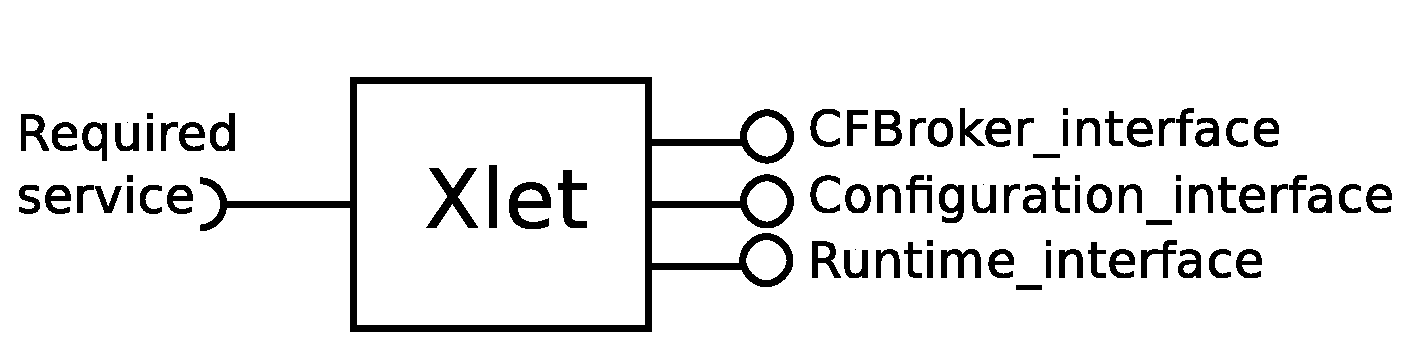
\includegraphics[width=0.6\textwidth]{pics/Xlet}
\caption{\label{fig:xlet} Xlet generic design}
\end{figure}

All Xlets respect the same architecture but differs in their implementations from a use case to another. In our current work we defined different monitoring and reporting Xlets. 
Monitoring Xlets are in-line with the DMTF standard. They allow collecting monitoring data for a specific type of resources with different granularities. For example, 
Figure~\ref{fig:slxlet} shows a SoftLayer specific Xlet. SLXlet allow to get monitoring data of SoftLayer provisioned servers for a given account. The account credentials are 
passed to the Xlet in the configuration phase through the Configuration interface. Afterwards, the Runtime interface of the Xlet could be used to get the list of servers, the list 
of metrics for a given server or, the value for a given metric for a specific server.

\begin{figure}[H]
\centering
\hspace{1.5cm}
\includegraphics[width=0.7\textwidth]{pics/SLXlet}
\caption{\label{fig:slxlet} SoftLayer Xlet design}
\end{figure}

Using Xlets within Bluemix PaaS has been very helpful. The advantageous characteristics of using Xlets in this environment are the following:
\begin{itemize}
 \item Scalability: this characteristic is inherited from the scalability of Bluemix environment. Since the Xlet could be provisioned as an application or a service within 
Bluemix, it is easy to scale it horizontally to cope with the work load by adding or removing new instances,
\item Reusability: all Xlets have a common and generic core code that allow the easy reusability with minor modifications for specific use case, 
\item Manageability: managing Xlets is handled to Bluemix, the management here includes provisioning, deprovisioning, binding and unbinding Xlets to other applications,
\item Flexibility: Xlets could be integrated easily using Bluemix services, they could be provisioned using different plans (e.g., shared or dedicated). 
\end{itemize}

\bibliographystyle{splncs}

\bibliography{mainDoc}

%----------------------------------------------------------------------------------------


\end{document}
